% vim: tw=80

\chapter{Reconstruction of Jets}
\label{sec:jet_reconstruction}

In scattering processes with large momentum transfers, the outgoing partons
produce a collimated stream of particles when hadronizing. The clusters of these
particles are the experimental signatures of quarks and gluons in the detector
and are called \emph{jets}. Jets show up in the \CMS detector as a localized
deposit of energy in the calorimeters accompanied by a large number of tracks in
the direction of the deposited energy. Jets are reconstructed using different
techniques based on the amount of information available. If the jets are
reconstructed from the energy clusters within the calorimeters, they are called
\emph{calorimeter jets}. If the jet reconstruction uses particle flow
candidates, these are called \emph{particle flow jets}. By removing pile-up
tracks from the particle flow candidates before the jet clustering, one yields
\emph{particle flow CHS jets}. Later on, when talking about jets in the physics
analysis, it is always referred to particle flow CHS jets if not stated otherwise.

\section{The Particle Flow Algorithm}
\label{sec:particle_flow_algorithm}

\CMS uses the particle flow reconstruction
algorithm~\cite{CMS-PAS-PFT-09-001,CMS-PAS-PFT-10-001} to identify and
reconstruct particles by combining information from all detector
subsystems. Due to its compact design inside the solenoid, the hadronic
calorimeter is not able to stop and measure all particles which reduces the
energy resolution. However, taking into account the additional information of
the tracking system within the particle flow algorithm enhances the
reconstruction performance and leads to a jet energy resolution comparable to
\ATLAS. A key element in the particle flow algorithm is the strong magnetic field
of \CMS which allows the precise distinction between neutral and charged hadrons. 

The ingredients of the particle flow algorithm are the
tracks and vertices, reconstructed from hits in the tracking detectors, the
deposited energy in the electromagnetic and hadronic calorimeters and the tracks
in the muon system. The reconstructed particles are classified as muons,
electrons, photons, charged hadrons or neutral hadrons. The combination of all
sub-detectors yields an optimal identification and measurement of their momentum
and energy.

The tracks are found using the Combinatorial Track Finder (CTF)
algorithm~\cite{Adam:2005cg} employed by \CMS. Based on these tracks, the primary
vertices in an event are identified. The electromagnetic and hadronic
calorimeters are divided into a grid of cells based on the detector granularity
to identify calorimeter cluster seeds. If there are seeds with an energy
exceeding a certain threshold, they are used in an iterative merging algorithm
to form particle flow clusters. The different elements of the detector
information are then linked together into particle flow building blocks based on
the geometry and \chisq fits. At first, muons, which can be well identified
using the tracks in the muon detector, are reconstructed using the building
blocks connected to the muon system. Blocks connecting the inner
tracking system with the ECAL clusters are used to identify electrons.
Similarly, charged hadrons are identified using links between the
tracking system and the remaining calorimeter clusters. Only neutral objects
which leave no traces in the tracking system, remain. ECAL clusters are
interpreted as photon candidates, while the remaining HCAL clusters are assumed
to be deposits of neutral hadrons. To avoid any kind of double-counting of
energy, all particle flow building blocks of successfully reconstructed particle
candidates are removed and the energy of the calorimeter clusters is recalculated.

Finally, a set of so-called particle flow candidates is yielded. They consist of
well identified particles, which profit from the improved resolution gained by
the inclusion of tracking information. This collection of particles is then
used to reconstruct the jets and further physical objects.

\todo{Jetbild?/pf bild}

\section{Jet Algorithms}
\label{sec:jet_algorithms}

The information of the clustered stream of particles, also known as jets,
provides the link between the short-scale physics and the final-state
observations. There are many different algorithms available which cluster jets
from a set of input objects. Both \CMS and \ATLAS rely on the \antikt and
inclusive-\kt jet algorithms, which proved to be very robust and both are
collinear and infrared safe, see Section~\ref{sec:coll_safety}. They are
sequential recombination algorithms and combine the input objects based on a
distance measure in Minkowski space. All jets were reconstructed using the
efficient algorithms implemented in the FastJet library~\cite{Cacciari:2011ma}.

\subsection{Collinear and Infrared Safety}
\label{sec:coll_safety}

Hard partons undergo many collinear splittings in the fragmentation process.
Additionally, there are always emissions of soft particles in QCD-like events
caused by non-perturbative and perturbative effects. The reconstructed jets
should be insensitive to all these effects. Furthermore, fixed-order pQCD
calculations are associated with divergent tree-level matrix elements and the
corresponding loop level matrix elements. While these divergences cancel for
infrared safe and collinear safe jet algorithms, this is not guaranteed for jet
algorithms not fulfilling the infrared and collinear safety requirements.
Fig.~\ref{fig:infrared_safety} shows the effect of a collinear splitting (right
plot) and of additional soft particles (left plot) on the results of an unsafe
jet algorithm. Most of the cone-based jet algorithms which cluster elements
by employing a constant distance measure in the $\eta-\phi$ space are affected by the
previously mentioned issues. This leads to the popularity of the modern sequential
recombination algorithms which are used in almost all of todays jet-based
analyses.

\begin{figure}[htb]
    \centering
    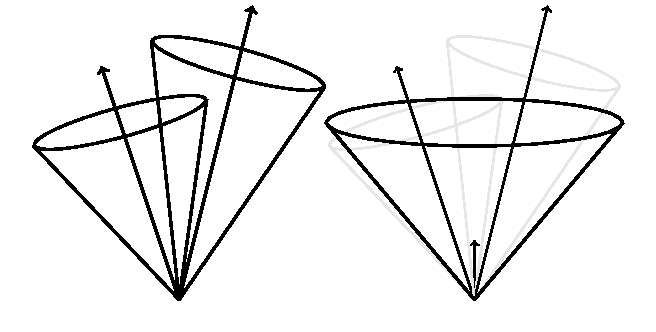
\includegraphics[width=0.45\textwidth]{figures/drawings/infrared_safety/jetinfrared.pdf}\hfill
    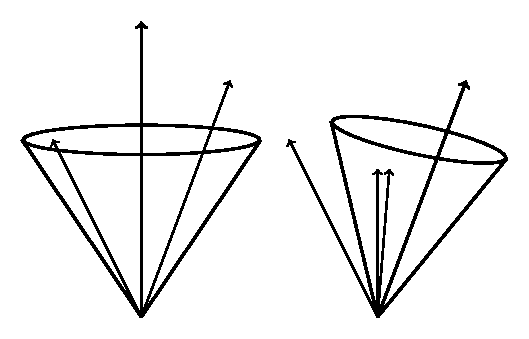
\includegraphics[width=0.45\textwidth]{figures/drawings/infrared_safety/jetcollinear.pdf}
    \caption[Effect of infrared emissions and collinear splittings on jet
    algorithms]{The influence of an infrared emission and a quasi
        collinear splitting on a jet algorithm not fulfilling the infrared safe
        and collinear safe requirements is shown. An additional soft particle (left plot)
    leads to the combination of the two jets into one large jet. A
quasi-collinear splitting of a particle (right plot) changes the result of the
jet clustering algorithm.}
    \label{fig:infrared_safety}
\end{figure}

\subsection{Generalized \kt Jet Algorithm}

The most popular sequential recombination algorithms are the \kt jet
algorithms which cluster jets based on a jet size parameter $R$ and an
additional parameter $p$, introducing a dependence on the transverse momentum of
the input objects. The pair-wise algorithm uses a list of input objects like stable
particles or particle flow candidates. 

At first, the distance $d_{ij}$ between two particles and the distances of the
particles to the beam $d_{iB}$ and $d_{jB}$ are calculated based on the rapidity
difference $\Delta y_{ij}$ and the azimuthal angle $\Delta \phi_{ij}$ between two
particles $i$ and $j$

\begin{align*} 
    d_{ij} &= \min(p_{\mathrm{T}i}^{2p},p_{\mathrm{T}j}^{2p})\frac{\left(\Delta
        R_{ij}\right)^2}{R^2}\\
    d_{i\mathrm{B}} &= k_{\mathrm{T}i}^{2p}
\end{align*} 

with the angular distance

\begin{align*}
    \left(\Delta R_{ij}\right)^2 &= (\Delta y_{ij})^2 + (\Delta \phi_{ij})^2
\end{align*} 

If distance $d_{ij}$ is smaller than the distances to the beam line, the two
particles $i$ and $j$ are merged into a new particle $k$ which then replaces the
particles $i$ and $j$ in the input list. These steps are repeated until all
particles are clustered into jets. Since the distance measures are defined in
Minkowski space, the shapes of the jets in the $\eta-\phi$ plane are not circular but
irregular, see Figure~\ref{fig:jet_shapes}. Based on the parameter $p$, there
are three important \kt based algorithms with distinct properties

\begin{figure}[htb]
    \centering
    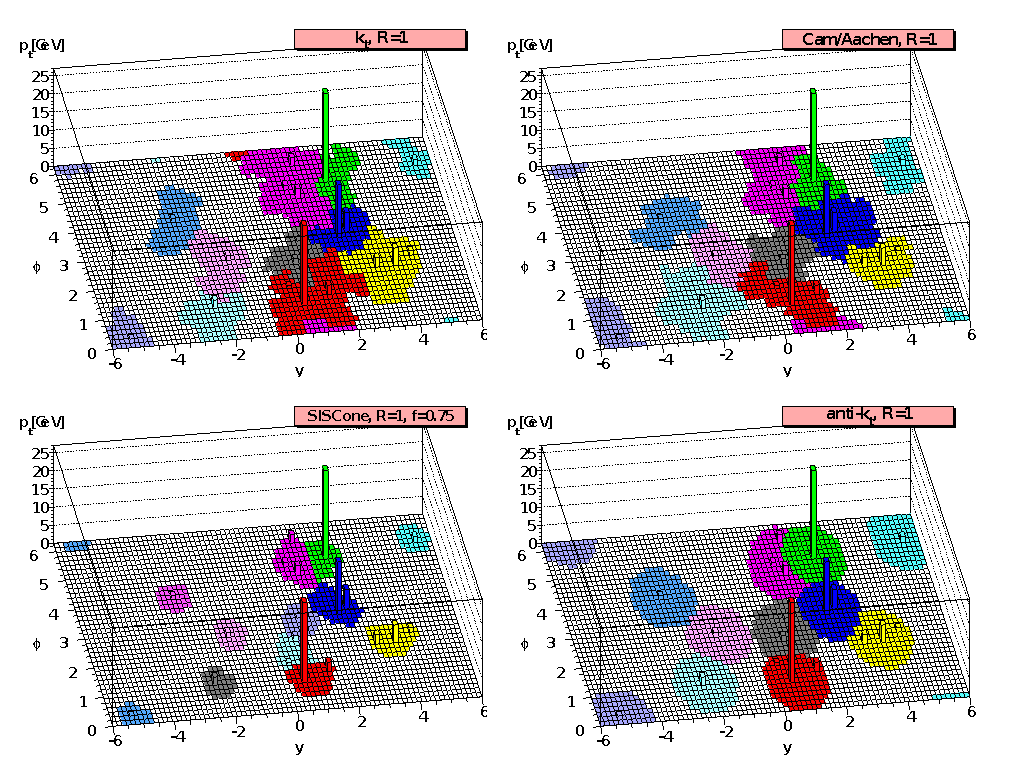
\includegraphics[width=0.8\textwidth]{figures/jet_reconstruction/jet_shapes.pdf}
    \caption[Jet areas of various jet algorithms]{The figure shows jet areas obtained by the described \kt based algorithm
        and the cone-based SISCone algorithm~\cite{Salam:2009jx}. For most jet
        algorithms the shape is irregular, while the \antikt algorithm yields
        circular shapes for hard jets while soft jets are crescent shaped.}
    \label{fig:jet_shapes}
\end{figure}

\begin{itemize}
    \item $p=1$: The \textbf{Inclusive $\mathbf{\kt}$
    algorithm}~\cite{Catani:1991hj,Catani:1992rm} is based on a \ptsq
        distance measure and approximately describes the inversion
        of the QCD branching process.
    \item $p=0$: The \textbf{Cambridge-Aachen
        algorithm}~\cite{Dokshitzer:1997in} is only based on the
        spatial separation of the objects and does not rely on the energy of
        the input objects. Similarly to the inclusive \kt algorithm its jets
        have an irregular shape. This jet algorithm is particularly interesting
        for jet substructure studies.
    \item  $p=-1$: The \textbf{anti-$\mathbf{\kt}$ algorithm}~\cite{Cacciari:2008gp} favours clustering hard input
        objects resulting in fairly circular jet shapes for hard jets, while
        soft jets are crescent-shaped if they are close to a hard jet.
\end{itemize}

\subsection{Jet Area}

The jet area describes the space covered by a jet object in the $\eta$-$\phi$
plane~\cite{Cacciari:2008gn}. While cone-based jet algorithms yield a $\pi R^2$
size area, the area for sequential jet algorithms needs to be determined for
each jet. A large number of infinitely soft particles, so-called ghost
particles, are evenly distributed in the event. The area $A_j$ of a jet $j$ is
assumed to be proportional to the number of ghost particles clustered into the
jet. 

The concept of jet areas is especially important in the context of pile-up
mitigation. The average \pt density $\rho$ in an event is estimated using the inclusive
\kt algorithm which also clusters many soft jets in the event and covers the
entire $\phi$-$\eta$ phase space. The average \pt density is defined as

\begin{equation*}
    \rho = \text{median} \frac{\pt^j}{A_j}
\end{equation*}

$\rho$ is a measure for the underlying event and pile-up activity in the event
and is used later on to correct the jets for these effects, see
Sec.~\ref{pileup_correction}.

\subsection{Charged Hadron Subtraction}
\label{sec:chs_algorithm}

\CMS introduced a new technique to reduce pile-up from jets using the high
resolution of the tracker, called Charged Hadron Subtraction
(CHS)~\cite{Kirschenmann:2014dla}. Naturally the CHS algorithm can only be
applied on jets within the tracker coverage of $|\eta| < 2.4$. All tracks of
particle flow candidates which originate from a pile-up vertex are removed.
Tracks originating from the main vertex or tracks not associated to any vertex
remain in the event. The jets are clustered from this set of particles.
Since the jet identification criteria in the jet selection in the analysis
require at least one charged particle in a jet, the CHS method is effectively
reducing the influence of pile-up on real jets as well as completely removing a
majority of the pile-up jets in the barrel region of the \CMS detector in
combination with the jet identification criteria.

The analysis presented in this thesis relies on CHS jets. Especially in the
low-\pt region, removing pile-up jets mimicking the leading jet in the event
improves the signal efficiency in the forward region.
\todo{joram chs bild}

\section{Jet Energy Corrections}
\label{sec:jec}
\todo{jec paper ref}

A detailed understanding of the jet energy scale and the jet transverse momentum
resolution is important when it comes to drawing conclusions about the
properties of quarks and gluons produced in high-energy scattering processes. On the
experimental side, there are multiple effects causing the reconstructed jet
energy not to correspond to the true jet energy like electronic noise, pile-up
and underlying event effects, but also non-linearities in the calorimeter
response and numerous further small effects. The jet reconstruction and
definition itself also introduces effects due to the fragmentation model,
initial- and final-state radiation which can cause out-of-cone effects.

The jet energy corrections (JEC) relate the measured jet energy to the
corresponding true particle jet energy. \CMS uses a factorized correction approach
consisting of multiple correction steps that build on one another. The corrected
transverse momentum $\pt^{\mathrm{corr}}$ of a jet is yielded by subsequently applying all correction
factors on an uncorrected jet

\begin{equation*}
    \pt^{\mathrm{corr}} = c_{\mathrm{res}} (\eta, \pt^{\prime}) \cdot c_{\mathrm{mc}}
    (\eta, \pt^{\prime\prime}) \cdot c_{\mathrm{pileup}}(\eta, \rho, A_j,
    \pt^{\mathrm{raw}}) \cdot \pt^{\mathrm{raw}},
\end{equation*}

\todo{switch to $p_{\mu}$?}

where $\pt^{\mathrm{raw}}$ is the transverse momentum of the uncorrected jet,
$\pt^{\prime}$ is the transverse momentum after applying the pile-up correction
factor $c_{\mathrm{pileup}}$. $\pt^{\prime\prime}$ is the transverse momentum
after the additional correction $c_\mathrm{MC}$ of relative and absolute effects
derived from MC studies. Finally a correction for residual effects
$c_{\mathrm{res}}$ derived from data is applied to yield the corrected jet
transverse momentum.

\paragraph{Pile-up Corrections}
\label{pileup_correction}

The first step removes the effects of pile-up contamination. Additional soft
proton-proton interactions produce particles being clustered into the jets
originating from the hard interaction. This additional amount of energy needs to
be subtracted by the pile-up correction. The applied correction is based on the
jet area method by using the pile-up density $\rho$ in the event and the jet
area $A_j$. The raw jet energy is then corrected by a factor proportional to the
pile-up density and the jet area.

\paragraph{MC Corrections}

Based on simulated QCD events, the jet energy scale is further corrected. The
momentum of a reconstructed jet can differ from a generated particle jet due to
out-of-cone effects or detector inefficiencies, which are modeled by the detector
simulation. The inverse response of the reconstructed jet to a generated jet is
applied as correction to remove these effects.

\paragraph{Residual Data Corrections}

Additional effects which can not be reliably estimated in a Monte Carlo
simulation are corrected for using data-driven methods. This correction step is
only applied on data. The relative residual corrections are based on
well-balanced dijet events in which a forward probe jet is calibrated using a
tag jet in the well understood barrel region. The last correction step is the
absolute residual correction in which reconstructed Z~bosons balanced to a jet
are used to calibrate the jet energy using the very precisely reconstructed Z~boson.

